Ontologias da web semântica e \foreignlanguage{english}{DSLs} têm
um papel fundamental na criação de um meio de descrição de conhecimento
por parte dos especialistas e no design de um framework para criação
de SADs. 

Ontologias servem para representar o conhecimento de especialistas
do domínio e DSLs servem para customizar o comportamento dos SADs.
Estas apareceram originalmente no contexto da filosofia, onde se referem
ao estudo da natureza, existência e realidade dos entes. Elas são
usadas em vários campos do conhecimento. Neste projeto, ontologias
referem-se a representações de conhecimento, que precisam ser implementadas
em código. As implementações de software podem trabalhar com ontologias
da Web Semântica que fornecem a criação, armazenamento, busca e modificação
de ontologias, seguindo padrões de formatos abertos. 

Neste capítulo, vamos apresentar e discutir as ontologias da web semântica
e as DSLs. Descrevendo a teoria da Web Semântica: fundamentos, Ontologias,
o \foreignlanguage{english}{Resource Description Framework (RDF}\nomenclature{RDF}{Resource Description Framework})
e a \foreignlanguage{english}{Web Ontology Language} (\foreignlanguage{english}{OWL}).
Finalmente serão abordadas as \foreignlanguage{english}{Domain Specific
Languages (DSLs}) que são linguagens que permitem definir um meio
de comunicação entre os especialistas e o sistema desenvolvido.

\section{Web Semântica.}

A web foi criada para possibilitar o acesso, intercâmbio e recuperação
de informações de maneira rápida e simples, seu crescimento exponencial
e caótico fez com que a mesma se tornasse hoje um gigantesco repositório
de documentos, o que dificulta a recuperação de informações. Até o
momento, não existe nenhuma estratégia abrangente e satisfatória para
a organização de documentos por meio de “motores de busca” que seja
coerente com uma estrutura linguística. \citep{Souza:2004}.

Um exemplo da deficiência da web atual, pode ser identificada na busca
realizada pelos sistemas de recuperação de informação, que usam palavras-chave
nas buscas, onde apenas a similaridade e o número de ocorrências de
certas palavras no conteúdo de documentos são levados em consideração
e não a semântica presente naquela informação. \citep{Souza:2004}.

A Web Semântica aparece como uma proposta para organizar o conhecimento
da internet semanticamente em formatos entendíveis pelos humanos e
máquinas \citep{bernerslee2001}. Procurando métodos para que as máquinas
consigam realizar a interpretação do significado, que é uma habilidade
inata dos seres humanos, através da associação dos conceitos que estão
no cérebro por meio de estruturas neurais e que não é suportado pelas
máquinas tradicionais.

A Web Semântica tem como finalidade estruturar os dados e informações
disponíveis na Web, para que tenham significado e sejam computáveis
por máquinas. Gerando um ambiente onde agentes de software e usuários
possam trabalhar de maneira cooperativa. A Web Semântica é definida
por um conjunto de padrões propostos pelo \foreignlanguage{english}{World
Wide Web Consortium} (W3C \nomenclature{W3C}{World Wide Web Consortium}).
A figura \ref{fig:Semantic_Web_History} apresenta alguns dos padrões
que constituem a Web Semântica de maneira cronológica. 

\begin{figure}[H]
\begin{centering}
\includegraphics[width=1\columnwidth]{\string"figures/Semantic Web History\string".eps}
\par\end{centering}
\caption{História da Web Semântica \label{fig:Semantic_Web_History}}

\fadaptada{bikakis2013xml}
\end{figure}

\citet{bernerslee2001} propuseram a Web Semântica, em 2001, como
uma extensão da Web atual, na qual é possível vincular conceitos de
maneira estruturada e padronizada. Permitindo a criação de conhecimento
estruturado, computável por máquinas, que pode ser compartilhado entre
humanos e máquinas. A finalidade é criar uma web universal dos conhecimentos
da humanidade. 

A partir dessa visão conceitual sobre a Web, \citet{bernerslee2001}
propuseram uma arquitetura que organiza as representações do conhecimento
por meio de camadas, conhecida como \foreignlanguage{english}{Semantic
Web Cake,} que é ilustrada na Figura \ref{fig:Web-Semantic-Architecture}.

\begin{figure}[H]
\begin{centering}
\includegraphics[width=0.6\columnwidth]{\string"figures/Semantic Web Architecture\string".eps}\caption{Arquitetura em camadas da Web Semântica\label{fig:Web-Semantic-Architecture}}
\par\end{centering}
\fadaptada{fensel2011semantic}
\end{figure}

A base dessa arquitetura é estabelecida pelos padrões \foreignlanguage{english}{Unicode}
e \foreignlanguage{english}{Uniform Resource Identifier} (URI\nomenclature{URI}{Uniform Resource Identifier}),
que padronizam a representação dos dados por meio das seguintes camadas: 
\selectlanguage{english}%
\begin{description}
\item [{Unicode}] \foreignlanguage{brazil}{é um padrão que codifica os
caracteres na maioria dos sistemas de escrita para representação de
texto com fines de processamento computacional.}
\item [{URI}] \foreignlanguage{brazil}{permite identificar os recursos
disponíveis na Web por meio de uma }String\foreignlanguage{brazil}{
única.}
\item [{XML}] \foreignlanguage{brazil}{representa os dados de maneira sintática,
através da definição de }markups\foreignlanguage{brazil}{ que codificam
documentos em formatos preestabelecidos. Ela permite que informações
sejam legíveis tanto por humanos como por computadores, suportando
as camadas superiores na arquitetura.}
\item [{RDF}] \foreignlanguage{brazil}{é um modelo padrão para intercambiar
dados na web. }RDF\foreignlanguage{brazil}{ tem características que
permitem a integração de dados inclusive de esquemas diferentes, e
suporta especialmente a evolução dos esquemas a través do tempo sem
requerer que mudanças nos consumidores de dados. A W3C especifica
ele }\footnote{\selectlanguage{brazil}%
\url{https://www.w3.org/RDF/}\selectlanguage{brazil}%
}\foreignlanguage{brazil}{.}
\item [{Ontology}] \foreignlanguage{brazil}{estende a camada de descrição,
fornecendo mais expressividade na definição de conceitos, de classificações,
de relações e de inferência.}
\item [{Logic}] \foreignlanguage{brazil}{permite definir regras lógicas
para deduzir e inferir novas informações que conseguem mudar a estrutura
da ontologia de maneira dinâmica.}
\item [{Proof}] \foreignlanguage{brazil}{fornece mecanismos para avaliar
o nível de confiabilidade das fontes de recursos e informações.}
\item [{Trust}] \foreignlanguage{brazil}{representa o conhecimento validado
e confiável.}
\item [{Digital-Signature}] \foreignlanguage{brazil}{permite integrar métodos
de segurança que garantam a segurança da informação.}
\end{description}
\selectlanguage{brazil}%
Uma das contribuições importantes da Web Semântica foi a formalização
da representação de ontologias (próxima sessão). No desenvolvimento
desta pesquisa, foram usadas desde as camadas inferiores até o \foreignlanguage{english}{OWL},
permitindo definir ontologias que representam os domínios de conhecimento.

\subsection*{Ontologias}

Existem várias interpretações do conceito ontologia, dependendo da
finalidade para qual elas sejam usadas. \citet{Smith2007} descrevem
a ontologia como uma área da filosofia, que estuda a natureza, existência
e realidade dos entes, assim como as categorias do ser e das relações
semânticas.

Na ciências da computação e informação, a palavra ``ontologia''
é definida como uma especificação formal e explicita de uma conceitualização
compartilhada de um domínio de conhecimento. \citet{allemang2011semantic}
definem as ontologias, no contexto da Web Semântica, como um esquema
de representação que permite conceitualizar e estruturar conhecimento,
permitindo a sua interpretação por computadores, com o objetivo de
compartilhar conhecimento entre humanos e computadores.

Uma ontologia é um sistema de organização e representação do conhecimento,
do inglês \foreignlanguage{english}{Knowledge Organization System
(KOS)}, que é uma estrutura conceitual e computacional que permite
representar o conhecimento, de qualquer domínio, por meio de entidades,
classificações, relações semânticas, regras e axiomas. Uma ontologia
é especificada por meio de componentes básicos que são as classes,
relações, axiomas e instâncias. 
\begin{description}
\item [{Classes}] são o foco da maioria das ontologias. Elas são utilizadas
para descrever os conceitos de um domínio, possibilitando a organização
e classificação dos indivíduos em um sistema lógico e hierárquico,
contendo subclasses que representam conceitos específicos \citep{noy2001ontology}. 
\item [{Relações}] representam o tipo de interação entre os conceitos de
um domínio e as propriedades presentes nas classes e indivíduos. Elas
podem ter características próprias, como serem transitivas, simétricas,
ou terem uma cardinalidade definida. 
\item [{Axiomas}] são utilizados para modelar regras assumidas como verdadeiras
no domínio em questão, de modo que seja possível associar relacionamentos
entre os indivíduos, além de fornecer características descritivas
e lógicas para os conceitos. 
\item [{Indivíduos,}] ou instâncias das classes, são utilizados para representar
elementos específicos, ou seja, os próprios dados, que juntamente
com a definição de uma ontologia, constituem a base de conhecimento
\citep{noy2001ontology}. Indivíduos representam objetos do domínio
de interesse \citep{horridge2011owl}.
\end{description}
Segundo \citet{Patel-schneider05buildingthe}, a representação de
uma ontologia é feita por meio de lógica de predicados e lógica descritiva,
usando padrões adotados pela comunidade, como \foreignlanguage{english}{RDF}
e \foreignlanguage{english}{OWL}. A Figura \ref{fig:Smart-data-continuum}
mostra os níveis de representação de dados na forma de conhecimento
processável por máquinas.

\begin{figure}[H]
\centering{}\includegraphics[width=0.6\columnwidth]{\string"figures/smart data\string".eps}\caption{\foreignlanguage{english}{Smart data continuum\foreignlanguage{brazil}{: níveis de representação
de dados na forma de conhecimento processável por máquinas.\label{fig:Smart-data-continuum}}}}
\end{figure}

O nível mais baixo de representação começa com os dados sem nenhum
significado semântico, dependentes do contexto da aplicação. O segundo
nível envolve a definição de esquemas \foreignlanguage{english}{XML}
para conseguir independência dos dados da aplicação, os dados fluem
entre aplicações em um único domínio mas não podem ser compartilhados
fora do domínio. No terceiro nível, os dados podem ser combinados
a partir de diferentes domínios, sendo suficientemente independentes
para serem recuperados e combinados com outras fontes de dados. Finalmente
no quarto nível, é possível inferir novos dados a partir dos existentes
e compartilha-los entre aplicações sem requerer interferência humana
\citep{sugumaran2011}.
\selectlanguage{english}%

\subsection*{Resource Description Framework\foreignlanguage{brazil}{ (}RDF\foreignlanguage{brazil}{)}}

\selectlanguage{brazil}%
O \foreignlanguage{english}{Resource Description Framework (RDF)}
é uma família de especificações da W3C, que foi disponibilizada em
1999 como parte do W3C's \foreignlanguage{english}{Semantic Web Effort}.
Elas fornecem um \foreignlanguage{english}{framework} comum que permite
que dados sejam compartilhados e reusados através das fronteiras das
aplicações, empresas e comunidades \footnote{\url{http://www.w3.org/2001/sw/}}.
O \foreignlanguage{english}{RDF} foi originalmente projetado como
um modelo de metadados e também chegou a ser usado como um método
de descrições conceituais, principalmente para descrever recursos
web e formalmente é um formato de dados de tipo grafo direcionado
e rotulado para representar informação na web\footnote{\url{https://www.w3.org/TR/rdf-sparql-query/}}.

O \foreignlanguage{english}{RDF} é usado em várias áreas de aplicação,
como \foreignlanguage{english}{\emph{resource discovery}}, para melhorar
as capacidades dos motores de busca, \foreignlanguage{english}{\emph{cataloging}},
para descrever conteúdo e as relações de conteúdo disponibilizados
em um sistema web particular, e descrição de \foreignlanguage{english}{\emph{intellectual
property rights}} de páginas web. Seu modelo básico de dados consiste
em um padrão de três tipos de objetos, conhecido como triplas\label{triplas}:
\begin{itemize}
\item \textbf{Sujeito}: representa os recursos e são identificados por meio
de \foreignlanguage{english}{URIs}. Por exemplo, uma página web ou
um elemento \foreignlanguage{english}{HyperText Markup Language (HTML
\nomenclature{HTML}{HyperText Markup Language})} podem ser recursos.
\item \textbf{Predicado}: são aspectos, características, atributos ou relações
especificas que descrevem o sujeito, cada predicado têm um significado
especifico e relaciona um sujeito com um objeto.
\item \textbf{Objeto}: um recurso especifico ou valor de propriedade que
representa uma características do sujeito \footnote{http://www.w3.org/TR/PR-rdf-syntax/}
\end{itemize}
Com \foreignlanguage{english}{RDF} é possível explicitar relações
entre dois objetos (usando-se uma Tripla \foreignlanguage{english}{RDF}),
mas não é possível fazer modelagens especificas nem inferência. Para
descrever detalhadamente o que um objeto representa e suas relações
com outros objetos, são necessárias ontologias descritas no padrão
\foreignlanguage{english}{OWL}. 
\selectlanguage{english}%

\subsection*{SPARQL Protocol and RDF Query Language (SPARQL\nomenclature{Sparql}{SPARQL Protocol and RDF Query Language})}

SPARQL\foreignlanguage{brazil}{ é uma linguagem de consulta semântica
usada por bancos de armazenamento e recuperação de dados de dados
compatíveis com o formato }RDF\foreignlanguage{brazil}{ ou que sejam
fornecidos como }RDF\foreignlanguage{brazil}{ via }middleware\foreignlanguage{brazil}{.
Atualmente é um padrão especificado pela }W3C\foreignlanguage{brazil}{
e uma das tecnologias principais da web semântica.}

\selectlanguage{brazil}%
A versão de SPARQL 1.1, veio com novas características que permitem
a atualização de dados em formato \foreignlanguage{english}{RDF},
permitindo atualizar, criar e remover dados em formato \foreignlanguage{english}{RDF}
em um \foreignlanguage{english}{Graph Store}\footnote{\url{https://www.w3.org/TR/sparql11-update/}}.
\selectlanguage{english}%

\subsection*{Web Ontology Language\foreignlanguage{brazil}{ (}OWL\foreignlanguage{brazil}{)}}

\selectlanguage{brazil}%
A \foreignlanguage{english}{Web Ontology Language} (\foreignlanguage{english}{OWL})
foi recomendada pelo W3C em 2004 para representar e compartilhar ontologias
na Web. Essa linguagem foi projetada para aplicações que necessitam
processar o conteúdo da informação, em vez de apenas organizar informações
em nós \citep{mcguinness2004owl}. \foreignlanguage{english}{OWL}
é uma linguagem que permite que a semântica seja explicitamente associada
ao conteúdo dos dados na web e formalmente especificada através de
ontologias, compartilhadas na Internet. 

A versão \foreignlanguage{english}{OWL} 2 é a versão mais recente
da linguagem. De acordo com as especificações do W3C\footnote{http://www.w3.org/TR/owl2-overview/},
a \foreignlanguage{english}{OWL 2} adicionou três novos perfis (\foreignlanguage{english}{sub-linguagens})
aos perfis DL e \foreignlanguage{english}{Full} já existentes: \foreignlanguage{english}{OWL
2} EL,\foreignlanguage{english}{ OWL 2 QL} e \foreignlanguage{english}{OWL
RL} (Figura \ref{fig:OWL2-Profiles}). Cada um desses perfis fornece
características de expressividade diferente para diversos cenários
de aplicação:

\begin{figure}[H]
\begin{centering}
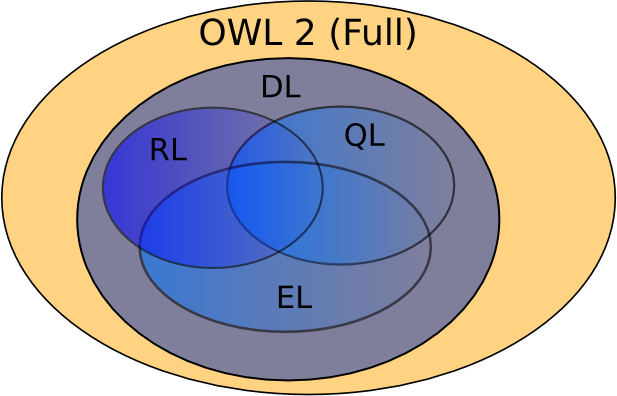
\includegraphics[width=0.6\columnwidth]{figures/owl2Profiles}
\par\end{centering}
\caption{OWL2 Profiles.\label{fig:OWL2-Profiles}}
\end{figure}

\selectlanguage{english}%
\begin{description}
\item [{Full}] \foreignlanguage{brazil}{O perfil }OWL Full\foreignlanguage{brazil}{
é direcionado para usuários que querem a máxima expressividade e a
liberdade sintática do }OWL\foreignlanguage{brazil}{ sem garantia
computacional. É improvável que qualquer motor de raciocínio seja
capaz de suportar completamente cada recurso da }OWL Full\foreignlanguage{brazil}{
\citep{mcguinness2004owl}.}
\selectlanguage{brazil}%
\item [{DL}] O perfil \foreignlanguage{english}{OWL DL} (\foreignlanguage{english}{Description
Logic}) é para aplicações que necessitam de máxima expressividade,
enquanto mantém a computabilidade (todas as conclusões são garantidas
de ser computáveis) e decidibilidade (todas as computações terminarão
em tempo finito) \citep{mcguinness2004owl}. \foreignlanguage{english}{OWL
DL} inclui as construções da linguagem \foreignlanguage{english}{OWL},
mas elas podem ser usadas somente sob certas restrições. 
\item [{EL}] O perfil \foreignlanguage{english}{OWL} 2 EL é baseado na
família EL++ de lógica descritiva (\foreignlanguage{english}{Description}
\foreignlanguage{english}{Logic}). Esse perfil é particularmente útil
em aplicações utilizando ontologias que contêm um grande número de
propriedades e/ou classes. Além disso, o \foreignlanguage{english}{OWL}
2 EL utiliza um padrão comum, utilizado em ontologias, para conceitos
e planejamento, ou seja, a combinação de conjunção e qualidades existenciais.
\selectlanguage{english}%
\item [{QL}] \foreignlanguage{brazil}{O perfil }OWL 2 QL\foreignlanguage{brazil}{
é baseado na família }DL-Lite\foreignlanguage{brazil}{ de lógica descritiva.
Esse perfil foi criado para permitir o raciocínio (}reasoning\foreignlanguage{brazil}{)
eficiente com grandes quantidades de dados estruturados de acordo
com esquemas relativamente simples. Ele fornece a maioria dos recursos
necessários para capturar modelos conceituais, tais como diagramas
de classe UML, diagramas de entidade/relacionamento, e esquemas de
banco de dados. }
\selectlanguage{brazil}%
\item [{RL}] O perfil \foreignlanguage{english}{OWL 2 RL} é voltado para
aplicações que exigem raciocínio escalável em troca de alguma restrição
de poder expressivo. Ele define um subconjunto sintático de \foreignlanguage{english}{OWL
2} que favorece a implementação utilizando tecnologias baseadas em
regras. Esse perfil pode ser utilizado na maioria das construções
\foreignlanguage{english}{OWL 2}. Porém, para permitir implementações
baseadas em regras de raciocínio, a forma como essas construções podem
ser usadas em axiomas foi restringida. 
\end{description}
\selectlanguage{brazil}%

\subsection*{Protégé}

O editor de ontologias Protégé \citep{musen2015protege}, é a ferramenta
recomendada pela comunidade para criar ontologias em formato \foreignlanguage{english}{OWL},
fornecendo:
\selectlanguage{english}%
\begin{itemize}
\item GUI Framework:\foreignlanguage{brazil}{ para suportar múltiplas vistas
da ontologia e layouts configuraveis de componentes.}
\item API:\foreignlanguage{brazil}{ para suportar o desenvolvimento de sistemas
baseados em conhecimento.}
\item Modularization\foreignlanguage{brazil}{: permite suportar a edição
de múltiplas ontologias em um mesmo entorno.}
\item Navigation\foreignlanguage{brazil}{: fornece buscas globais e locais
e hipervínculos nos editores.}
\item Refactoring tools\foreignlanguage{brazil}{: verificação de coerência
das ontologias.}
\item Reasoning:\foreignlanguage{brazil}{ compatibilidade com vários }reasoner\foreignlanguage{brazil}{
para suportar a inferência.}
\item Plug-ins\foreignlanguage{brazil}{: arquitetura extensível que suporta
diferentes tipos de }plug-ins.
\end{itemize}
\selectlanguage{brazil}%

\selectlanguage{english}%

\subsection*{Triplestore\label{subsec:Triplestore}}

\selectlanguage{brazil}%
Uma \foreignlanguage{english}{triplestore} é um tipo de banco de dados
baseado em grafos que armazena fatos semânticos, e fornece o armazenamento
e a recuperação de triplas no padrão \foreignlanguage{english}{RDF}
(Seção \ref{triplas}). Os dados são armazenados em forma de redes
de objetos com vínculos rotulados entre eles, \citep{rusher2003triple}.
Este tipo bancos de dados são recomendáveis quando os dados tem uma
estrutura flexível, cujas relações não tem um padrão definido.

A \foreignlanguage{english}{triplestore} \foreignlanguage{english}{Blazegraph}
\footnote{\url{https://www.blazegraph.com/}} é um dos mais completos
bancos de dados baseados em grafos e com suporte SPARQL. Ele integra
as características de uma \foreignlanguage{english}{triplestore},
fornece suporte nativo a \foreignlanguage{english}{SPARQL} e implementa
o \foreignlanguage{english}{SPARQL Protocol Endpoint}. Esse último,
padroniza a comunicação com os clientes e a compatibilidade com os
sistemas web, por meio de \foreignlanguage{english}{um Endpoint} (um
endereço onde requisições em SPARQL podem ser feitas). 

O Blazegraph foi escolhido por ter código aberto (Licença GPL) e ser
compatível com os padrões da Web Semântica. Mas qualquer \foreignlanguage{english}{triplestore}
que seja compatível com os mesmos padrões SPARQL 1.1 e RDF pode ser
usada. As principais características dele são:
\begin{itemize}
\item Banco de dado baseado em grafo de alta performance
\item Suporte Blueprints API e RDF/SPARQL
\item Clusters de replicação altamente disponíveis (HAJournalServer) 
\item Armazenamento de dados de uma única máquina até \textasciitilde{}50B
triples/quads (RWStore) 
\item O armazenamento de dados em cluster é essencialmente ilimitado (BigdataFederation) 
\item REST API Com deployment embutida e / ou webapp (NanoSparqlServer) 
\item SPARQL 1.1 nativo 
\item RDFS+ Inferência e manutenção da verdade
\item Triples, quads, ou Reificação feita corretamente (RDR) support 
\item Gerenciador de memória Java aproveita o JVM nativo heap (no GC) 
\item API centrada em vértices(RDF\_GAS\_API) 
\item Licença dupla: GPLv2 ou commercial 
\item Assinaturas de suporte ao desenvolvedor e produção
\end{itemize}

\subsection*{Discussão }

Para desenvolver os sistemas software da presente pesquisa foram usadas
tecnologias da web semântica. Primeiramente foram desenhadas as ontologias
em formato \foreignlanguage{english}{OWL} na ferramenta Protégé, depois
instanciadas em \foreignlanguage{english}{triplestores} e finalmente
integradas no framework Decisioner que está implementado sobre o banco
de dados baseado em grafos \foreignlanguage{english}{Blazegraph} .

\selectlanguage{english}%
Blazegraph\foreignlanguage{brazil}{ permitiu instanciar as ontologias
em formato }RDF,\foreignlanguage{brazil}{ suportar inferência e permitir
consultas através da linguagem }SPARQL,\foreignlanguage{brazil}{ suportando
a definição e atualização dos conceitos das ontologias. Estas funcionalidades
foram complementadas com ferramentas de edição da ontologia via web
e }real-time\foreignlanguage{brazil}{, esta implementação está descrita
no capítulo \ref{chap:Decisioner}. }

\selectlanguage{brazil}%
Além das ontologias, foi necessário fornecer um meio de definição
de conhecimento mais próximo à linguagem dos especialistas do domínio,
para suportar a definição de SADs por parte dos especialistas. A solução
identificada foi criar uma \foreignlanguage{english}{DSL} definida
a continuação.
\selectlanguage{english}%

\section{Domain Specific Language (DSL)\foreignlanguage{brazil}{ }}

\selectlanguage{brazil}%
Em desenvolvimento de software e engenharia de domínio uma linguagem
de domínio específico, em inglês \foreignlanguage{english}{\emph{Domain-Specific
Language}}\emph{ (DSL)}, é um tipo de linguagem de programação, ou
linguagem de especificação, dedicada a um domínio particular de problema
que usa expressões próprias dos especialistas daquele domínio. Um
usuário, relacionado com um domínio específico, pode usar uma DSL
sem ter experiência em desenvolvimento de software pois a DSL está
relacionada com seu domínio de trabalho. \citet{fowler2010domain}
afirma que programadores instruem o computador no que ele deve fazer,
pois já entendem a maneira dele trabalhar, mas com \foreignlanguage{english}{DSLs}
é feito o inverso: o computador começa a entender o que o usuário
do domínio escreve.

Segundo \citet{Mernik:2005:DDL:1118890.1118892}, as vantagens das
DSL, em comparação com as linguagens de propósito geral, são a expressividade,
facilidade de uso e a integração com o domínio da aplicação. O conceito
não é novo, linguagens de programação de propósito especifico existem
desde o começo das linguagens de programação, mas o termo tornou-se
padrão devido à ascensão da modelagem de domínio específico. DSLs
são classificadas da seguinte forma:
\selectlanguage{english}%
\begin{itemize}
\item Domain-Specific Markup Languages\foreignlanguage{brazil}{: são linguagens
de um domínio particular com a particularidade de anotar os dados
com etiquetas para que eles sejam sintaticamente distinguíveis. Um
exemplo delas é a }Hypertext Markup Language (HTML),\foreignlanguage{brazil}{
que permite anotar dados no domínio das páginas web.}
\item Domain-Specific Modeling Languages (specification languages):\foreignlanguage{brazil}{
são linguagens que permitem especificar sistemas com o propósito de
modelar eles, são compostos de uma estrutura consistente de um conjunto
de regras que permitem interpretar o significado dos componentes modelados.
Uma linguagem deste tipo é a }Unified Modeling Language\foreignlanguage{brazil}{
(}UML\nomenclature{UML}{Unified Modeling Language }\foreignlanguage{brazil}{)
que permite especificar sistemas de software.}
\item Domain-Specific Programming Languages:\foreignlanguage{brazil}{ são
linguagens que permitem a programação em alto nível aplicada a um
domínio especifico de conhecimento. Uma linguagem desse tipo é a linguagem
R que permite a programação de conceitos estatísticos e geração de
gráficos.}
\end{itemize}
\selectlanguage{brazil}%

Segundo o tipo de implementação as DSL podem ser dividas em \foreignlanguage{english}{external
DSL e internal DSL,} explicadas a continuação\citep{fowler2010domain}:

\selectlanguage{english}%
External DSL:\foreignlanguage{brazil}{ é uma linguagem de domínio
especifico que é definida com uma sintaxes independente de outras
linguagens de programação, tendo como principal vantagem a flexibilidade
da DSL. A desvantagem é que requer um desenvolvimento de um }full\foreignlanguage{brazil}{
parser para processar ela.}

Internal DSL:\foreignlanguage{brazil}{ é uma linguagem de domínio
especifico escrita dentro de uma linguagem }host\foreignlanguage{brazil}{
existente. A vantagem deste enfoque de definição de DSL é que o tempo
e custo de desenvolvimento é menor em relação a definir uma DSL externa.
Este tipo de linguagens são escritas sobre uma linguagem de propósito
geral e por isso apresenta a desvantagem da linguagem depender das
instruções e características da linguagem }host,\foreignlanguage{brazil}{
o que em alguns casos afeta a flexibilidade e expressividade da DSL
que quer-se definir.}
\selectlanguage{brazil}%

\subsection*{Linguagem \foreignlanguage{english}{Groovy}}

\selectlanguage{english}%
Groovy\foreignlanguage{brazil}{ é uma linguagem dinâmica para a máquina
virtual Java (}JVM\foreignlanguage{brazil}{) \citep{koenig2007groovy}.
Ela tem uma sintaxe parecida com Java, suporte para programação funcional,
produz }JVM bytecodes\foreignlanguage{brazil}{ e interopera bem com
código e bibliotecas Java. Traz características de linguagens como
}Python\foreignlanguage{brazil}{, }Ruby\foreignlanguage{brazil}{ e
}Smalltalk\foreignlanguage{brazil}{ para uma linguagem similar a Java
\citep{koenig2007groovy}.}

\selectlanguage{brazil}%
O grande benefício que \foreignlanguage{english}{Groovy} traz para
este projeto é o suporte que da natureza dinâmica que dá ao desenvolvimento
de DSLs. Essas DSLs podem rodar diretamente na \foreignlanguage{english}{JVM}
e usar bibliotecas Java já existentes. DSLs em \foreignlanguage{english}{Groovy}
se integram facilmente à própria linguagem Groovy de modo que não
é aparente onde o código em \foreignlanguage{english}{Groovy} termina
e a DSL começa \citep{dearle2015groovy}. Isso permite que a DSL
seja implementada como uma DSL interna, estendendo a linguagem Groovy
(e simplificando a sua criação), mas mantenha uma sintaxe próxima
à linguagem usada pelos especialistas de domínio. Como uma DSL interna,
ela pode usar ferramentas já existentes para auxiliar a escrita de
código em Groovy, como editores com \foreignlanguage{english}{\textit{syntax
highlighting}} e \foreignlanguage{english}{\textit{code completion}},
para a sua edição.

Outra vantagem de Groovy é que ela é uma linguagem para a \foreignlanguage{english}{JVM}
e existem muitas bibliotecas, em Java, que dão suporte às tecnologias
da Web Semântica. Isso inclui bibliotecas como a \foreignlanguage{english}{OWL
API}, para trabalhar com ontologias em \foreignlanguage{english}{OWL},
Apache \foreignlanguage{english}{Jena}, para acesso a \foreignlanguage{english}{triplestores},
entre outras. Finalmente, os SADs a serem criados serão aplicativos
web, Groovy tem um web framework completo e madurecido, Grails\foreignlanguage{english}{}\footnote{\selectlanguage{english}%
\url{https://grails.org/}\selectlanguage{brazil}%
}. 

Grails usa uma abordagem de convenção sobre configuração que usa opções
default razoáveis. Ele se integra bem com a JVM e tem características
como ORM integrado, DSLs, metaprogramação durante runtime e compile-time,
e programação assíncrona \citep{smith2009grails}.


\subsection*{Discussão}

A partir do análise dos especialistas do domínio foi determinado que
não têm um conhecimento detalhado sobre modelagem de conhecimento
usando os padrões da web semântica, descritos neste capítulo. 

Também foi determinado que as ontologias permitem uma definição detalhada
do conhecimento do domínio, pelo que foi necessário definir uma camada
intermédia que facilitasse a definição do conhecimento por parte dos
especialistas. Por isso foi identificado a necessidade de uma DSL
adequada ao nível de conhecimento de computação dos especialistas,
e que contenha termos familiares ao domínio desses especialistas. 

Uma DSL de tipo \foreignlanguage{english}{programming} pode suportar
a definição de conhecimento dos especialistas, fornecendo uma solução
compatível com os termos específicos deles. Isso facilita que os especialistas
especifiquem os SAD com um grau de detalhamento suficiente para definir
o conhecimento deles sem intervenção dos desenvolvedores de software,
os especialistas poderiam se tornar, na prática, programadores de
seus próprios SADs.

Neste projeto, DSLs servem para customizar o comportamento dos SADs.
Por isso, uma \foreignlanguage{english}{Domain-Specifc Programming
Language }foi desenvolvida. Ela faz uso da ontologia para organizar
o conhecimento do domínio e definir o comportamento dos SADs (Figura
\ref{fig:Componente-DSL}). Para facilitar a criação desse tipo de
DSL, a linguagem \foreignlanguage{english}{Groovy}\footnote{\selectlanguage{english}%
\url{http://groovy-lang.org/}\selectlanguage{brazil}%
} foi escolhida para implementação. 

\begin{figure}[H]
\begin{centering}
\includegraphics[width=0.5\columnwidth]{\string"figures/DSL Diagram\string".eps}
\par\end{centering}
\caption{Componente DSL \label{fig:Componente-DSL}}
\end{figure}


\section{Considerações finais}

A partir do problema identificado e da revisão da literatura foi encontrado
que o desenvolvimento de ontologias é um área de pesquisa abrangida
pela Web Semântica que permite desenvolver sistemas web baseados em
conhecimento, satisfazendo os requisitos de desenvolvimento do SAD
SustenAgro explicados no capítulo \ref{chap:SAD}.

Porém, a definição de uma ontologia não é uma tarefa trivial, pelo
que existe dificuldade por parte dos especialistas do domínio ao definir
as ontologias. Diante deste cenário foram analisadas varias soluções
e encontrou-se que complementando a ontologia com uma DSL, favorece
na definição dos conceitos dos especialistas em uma linguagem mais
natural para os especialistas.

A continuação será apresentado o capítulo intitulado ``Framework
Decisioner'' que faz uso das tecnologias explicadas para definir
um Framework que facilite a definição de conhecimento dos especialistas
com a finalidade de gerar SADs.
